%TODO Spell check
%TODO Have parameters handy for presentation
%TODO Print papers you want to take with you

%%%%%%%%%%%%%%%%%%%%%%%%%%%%%%%%%%%%%%%%%%%%%%%%%%%%%%%%%%%%%%%%%%%%%%%%%%%%%%
% Preamble {{{ 
%%%%%%%%%%%%%%%%%%%%%%%%%%%%%%%%%%%%%%%%%%%%%%%%%%%%%%%%%%%%%%%%%%%%%%%%%%%%%%

\PassOptionsToPackage{svgnames}{xcolor}
\documentclass[a0paper]{tudposter}

% Bei Bedarf: dinBold f�r Section. Dann aber auch �berschrift nur in
% Gro�buchstaben.
\addtokomafont{section}{\dinBold}

%% Verwendung von CM Bright f�r Formeln.
%\usepackage{cmbright}
%\renewcommand*{\sfdefault}{aun}
%\renewcommand*{\ttdefault}{aun}
%\normalfont

% In diesem Poster ben�tigte Pakete.
% Jedem wie es beliebt.
\usepackage[T1]{fontenc}
\usepackage[latin1]{inputenc}
\usepackage{multicol}
\usepackage{amsmath, amssymb}
\usepackage{dsfont}
\usepackage[ngerman]{babel}
\usepackage{relsize}
\usepackage{enumitem}
\usepackage{graphics, graphicx, tikz, cite}
\usepackage{tcolorbox, color}
\usepackage{array, blindtext}
\usepackage{multirow}

\tcbuselibrary{skins,breakable}
\usetikzlibrary{shadings,shadows}
\usetikzlibrary{arrows}

\usetikzlibrary{decorations,arrows} 
\usetikzlibrary{decorations.pathmorphing} 
\usepgflibrary{decorations.pathreplacing}

% Beschriftung im Seitenkopf und Seitenfu�
\pagestyle{tudposter}
\einrichtung{Fakult�t Mathematik und Naturwissenschaften}
\institut{Institut f�r Theoretische Physik}
\professur{Theoretische Quantenoptik}
\fusszeile{Please feel free to contact us at daniel.suess@mailbox.tu-dresden.de}% Zum Beispiel f�r Kontaktdaten.


\newcommand{\ket}[1]{| #1 \rangle}
\newcommand{\bra}[1]{\langle #1 |}
\newcommand{\Hel}{H_\mathrm{el}}
\newcommand{\opH}[1]{H_\mathrm{#1}}
\newcommand{\opHH}[1]{\mathcal{H}_\mathrm{#1}}
\newcommand{\ptr}{\mathrm{Tr}_\mathrm{env}}
\newcommand{\ii}{\mathrm{i}}
\newcommand{\adj}[1]{#1^{\dagger}}
\newcommand{\cc}[1]{{#1}^\ast}
\newcommand{\quotes}[1]{``#1''}
\newcommand{\dd}{\mathrm{d}}
\renewcommand{\vec}[1]{\mathbf{#1}}
\newcommand{\abs}[1]{\vert #1 \vert}


\newcommand{\zz}{{\vec z}}               % Our noise process
\newcommand{\ZZ}{\cc{Z}}               % Our noise process
\newcommand{\tildeZZ}{\cc{\tilde Z}}
\newcommand{\adjZZ}{\mathcal{D}}         % and it's adjoint

\newcommand{\E}[1][\empty]{%
  \ifthenelse{\equal{#1}{\empty}}
  {\mathbb{E}}
  {\mathbb{E}\left( #1 \right)}
}
\newcommand{\unit}{\mathrm{I}}

\renewcommand{\exp}[1][\empty]{%
  \ifthenelse{\equal{#1}{\empty}}
    {\mathrm{exp}}
    {\mathrm{e}^{#1}}
}

\newcommand{\braket}[2]{\langle #1 | #2 \rangle}


\newcommand{\psit}[1][\empty]{%
  \ifthenelse{\equal{#1}{\empty}}
    {\psi_t}
    {\psi_t^{(#1)}}
}
\newcommand{\psitz}[1][\empty]{%
  \ifthenelse{\equal{#1}{\empty}}
    {\psi_t(\cc\zz)}
    {\psi_t^{(#1)(\cc\zz)}}
}
\newcommand{\psitZ}[1][\empty]{%
  \ifthenelse{\equal{#1}{\empty}}
    {\psi_t(\ZZ)}
    {\psi_t^{(#1)}(\ZZ)}
}

\newcommand{\NMSSE}{\textsc{NMSSE}}

\setitemize[0]{leftmargin=20pt,itemindent=20pt}
\setitemize[2]{leftmargin=60pt,itemindent=20pt}
%% Test
% Ausdruck des linken oberen Seitenausschnitts auf A4.
% Zum Beispiel zur Kontrolle der Schriftart.
%\AtBeginDvi{\special{papersize=21cm,29.7cm}}% f�r A4
%}}}
%%%%%%%%%%%%%%%%%%%%%%%%%%%%%%%%%%%%%%%%%%%%%%%%%%%%%%%%%%%%%%%%%%%%%%%%%%%%%%
%%% Farbdefinitionen%{{{
%%%%%%%%%%%%%%%%%%%%%%%%%%%%%%%%%%%%%%%%%%%%%%%%%%%%%%%%%%%%%%%%%%%%%%%%%%%%%%
\definecolor{HKS41K100}{cmyk}{1.00, 0.70, 0.10, 0.50}
\definecolor{HKS41K90}{cmyk}{0.9, 0.63, 0.09, 0.45}
\definecolor{HKS41K80}{cmyk}{0.8, 0.56, 0.08, 0.40}
\definecolor{HKS41K70}{cmyk}{0.7, 0.49, 0.07, 0.35}
\definecolor{HKS41K60}{cmyk}{0.6, 0.42, 0.06, 0.30}
\definecolor{HKS41K50}{cmyk}{0.5, 0.35, 0.05, 0.25}
\definecolor{HKS41K40}{cmyk}{0.4, 0.28, 0.04, 0.20}
\definecolor{HKS41K30}{cmyk}{0.3, 0.21, 0.03, 0.15}
\definecolor{HKS41K20}{cmyk}{0.2, 0.14, 0.02, 0.10}
\definecolor{HKS41K10}{cmyk}{0.1, 0.07, 0.01, 0.05}
%}}}
%%%%%%%%%%%%%%%%%%%%%%%%%%%%%%%%%%%%%%%%%%%%%%%%%%%%%%%%%%%%%%%%%%%%%%%%%%%%%%
%%% Colored Blocks%{{{
%%%%%%%%%%%%%%%%%%%%%%%%%%%%%%%%%%%%%%%%%%%%%%%%%%%%%%%%%%%%%%%%%%%%%%%%%%%%%%

%TODO Choose color scheme for boxes 
\newenvironment{block}[1]{%
    \tcolorbox[skin=enhanced,
    frame style={drop shadow},
    noparskip,breakable,
    colback=white,colframe=HKS41K50,%
    colbacklower=white,%
    %Dirty trick to fix title-bar size
    title=\Large \dinBold #1 \color{HKS41K50} \huge yW,
    arc=0mm,
    boxrule=1mm
    ]}%
    {\endtcolorbox}

\newenvironment{block_wo_heading}{%
    \tcolorbox[
    noparskip,breakable,
    colback=white,colframe=white,%
    colbacklower=white,%
    arc=0mm,
    boxrule=.0mm
    ]}%
    {\endtcolorbox}

  %}}}
%%%%%%%%%%%%%%%%%%%%%%%%%%%%%%%%%%%%%%%%%%%%%%%%%%%%%%%%%%%%%%%%%%%%%%%%%%%%%%
%%% Emphasise Equations%{{{
%%%%%%%%%%%%%%%%%%%%%%%%%%%%%%%%%%%%%%%%%%%%%%%%%%%%%%%%%%%%%%%%%%%%%%%%%%%%%%

\usepackage{empheq}

\newlength\mytemplen
\newsavebox\mytempbox

\makeatletter
\newcommand\mybluebox{%
    \@ifnextchar[%]
       {\@mybluebox}%
       {\@mybluebox[0pt]}}

\def\@mybluebox[#1]{%
    \@ifnextchar[%]
       {\@@mybluebox[#1]}%
       {\@@mybluebox[#1][0pt]}}

\def\@@mybluebox[#1][#2]#3{
    \sbox\mytempbox{#3}%
    \mytemplen\ht\mytempbox
    \advance\mytemplen #1\relax
    \ht\mytempbox\mytemplen
    \mytemplen\dp\mytempbox
    \advance\mytemplen #2\relax
    \dp\mytempbox\mytemplen
    \colorbox{HKS41K10}{\hspace{1em}\usebox{\mytempbox}\hspace{1em}}  }
\makeatother

%}}}

\begin{document}
%%%%%%%%%%%%%%%%%%%%%%%%%%%%%%%%%%%%%%%%%%%%%%%%%%%%%%%%%%%%%%%%%%%%%%%%%%%%
%%% Poster-Titel%{{{
%%%%%%%%%%%%%%%%%%%%%%%%%%%%%%%%%%%%%%%%%%%%%%%%%%%%%%%%%%%%%%%%%%%%%%%%%%%%

  {\dinBold\veryHuge\color{HKS41K100} Energy transfer dynamics in structured environments} \\

\setlength{\tabcolsep}{0cm}
\begin{block_wo_heading}
  \begin{description}
    \item \LARGE Daniel S��, Walter T. Strunz
    \item \normalsize Institut f�r Theoretische Physik, Technische Universit�t Dresden, D-01062 Dresden, Germany
  \end{description}
  \begin{large}
  Our aim is to present a novel approach to the numeric treatment of open quantum systems similar to [1].
  On the basis of a stochastic Schr�dinger equation we develop a hierarchy of equations of motion which can be used to simulate their time evolution.
  This method is then applied to energy transfer dynamics and absorption spectra in molecular aggregates.
  \end{large}
  \vspace{1mm}
\end{block_wo_heading}


\raggedright

%}}}
%%%%%%%%%%%%%%%%%%%%%%%%%%%%%%%%%%%%%%%%%%%%%%%%%%%%%%%%%%%%%%%%%%%%%%%%%%%%
%%% Introduction%{{{
%%%%%%%%%%%%%%%%%%%%%%%%%%%%%%%%%%%%%%%%%%%%%%%%%%%%%%%%%%%%%%%%%%%%%%%%%%%%

\setlength{\tabcolsep}{0cm}
\begin{tabular}{p{.48\textwidth} p{.03\textwidth} p{.49\textwidth}}
\begin{block}{Non-Markovian quantum state diffusion}
\begin{itemize}
  \item stochastic Schr�dinger equation in the Hilbert space of the system [2]
  \begin{empheq}[box={\mybluebox}]{align*}
     \partial_t \, \psi_t = - i H \psi_t + L \cc{Z}_t \psi_t - \adj{L} \int_0^t \alpha(t-s) \,
     \frac{\delta \psi_t}{\delta \cc{Z}_s} \dd s
  \end{empheq}

  \begin{itemize}
    \vspace{.3cm}
    \setlength{\columnsep}{1cm}
    \begin{multicols}{2}
    \item free Hamiltonian $H$
    \item coupling operator $L$
    \columnbreak
    \item bath correlation function $\alpha$
    \item complex noise $Z_t$ with cov. $\alpha$
    \end{multicols}
  \end{itemize}

  \vspace{.3cm}
  \item equation for state vectors $\implies$ well suited for numerics
  \item density operator recovered as ensemble average over $Z_t$
  \item no approximation necessary so far
  \item[\raisebox{.2ex}{$\Rightarrow$}]Functional derivation? Time non-locality? \raisebox{.2ex}{$\implies$} \textbf{Hierarchical Equations!}
\end{itemize}
  \vspace{3.6mm}
\end{block}

&    &

\begin{block}{Hierarchical equations of motion}
\begin{itemize}
\item \textbf{Idea:} derive equation of motion for problematic term
  \begin{align*}
    \psi_t^{(1)} := \int_0^t \alpha(t-s) \, \frac{\delta \psi_t}{\delta \cc{Z}_s} \dd s
  \end{align*}
\item simple form only for exponential correlation function $\alpha(t) \propto \ee^{-\gamma \vert t \vert - \ii \Omega t}$
\item same structure as NMSSE, but with second order functional derivation
\item[\raisebox{.2ex}{$\Rightarrow$}] Infinite Hierarchy of state vectors $\psi_t^{(k)}$:
  \begin{empheq}[box={\mybluebox[5pt][7pt]}]{align*}
     \partial_t \, \psi_t^{(k)} =
     \left(  -\ii H - (\gamma + \ii \Omega)k + L \cc{Z}_t  \right) \psi_t^{(k)} 
      + k \alpha(0) L \psi_t^{(k-1)} 
      - \adj{L} \psi_t^{(k+1)}
  \end{empheq}
\item higher orders suppressed by $\ee^{-\gamma k}$ \raisebox{.2ex}{$\implies$} truncation for numerical treatment
\end{itemize}
\end{block}
\end{tabular}

%}}}
%%%%%%%%%%%%%%%%%%%%%%%%%%%%%%%%%%%%%%%%%%%%%%%%%%%%%%%%%%%%%%%%%%%%%%%%%%%%
%%% Main Part%{{{
%%%%%%%%%%%%%%%%%%%%%%%%%%%%%%%%%%%%%%%%%%%%%%%%%%%%%%%%%%%%%%%%%%%%%%%%%%%%

\raggedright
\begin{block}{Energy transfer and absorption spectra in molecular dimers}
\begin{tabular}{m{0.55\textwidth} m{0.45\textwidth}}


  \begin{center}
  \begin{tikzpicture}[scale=1.0]%{{{

    \draw [line width=0.1cm] (-10,5.5) -- (-8,5.5);
    \draw [line width=0.1cm] (-10,2) -- (-8,2);
    \draw [->, line width=.1cm, color=red] (-9,2.1) -- (-9,5.4);
    \node (text) at (-9,6.0) {\small $\vert e_1 \rangle$};
    \node (text) at (-9, 1.5) {\small $\vert g_1 \rangle$};
    \node (text) [color=red] at (-8.5,2.7) {$\epsilon$};
    \draw [line width=.02cm, dashed] (-9,3.8) ellipse (2.2 and 3);

    \draw [line width=.1cm] (-10.5,12) parabola[parabola height=-4cm] (-6.5,12);
    \draw [line width =.02cm] (-10,11) -- (-7.0,11);
    \draw [line width =.02cm] (-9.7,10) -- (-7.3,10);
    \draw [line width =.02cm] (-9.3,9) -- (-7.7,9);
    \draw [line width=.1cm, xshift=1cm, yshift=.7cm] (-10.5,12) parabola[parabola height=-4cm] (-6.5,12);
    \draw [line width =.02cm, xshift=1cm, yshift=.7cm] (-10,11) -- (-7.0,11);
    \draw [line width =.02cm, xshift=1cm, yshift=.7cm] (-9.7,10) -- (-7.3,10);
    \draw [line width =.02cm, xshift=1cm, yshift=.7cm] (-9.3,9) -- (-7.7,9);
    \node (text) at (-8,12.5) {$\alpha_1$};
    \draw [<->, line width=0.1cm, color=blue] (-8.7,7.9) -- (-9.0,6.9);


    \draw [line width=0.1cm] (-4,5.5) -- (-2,5.5);
    \draw [line width=0.1cm] (-4,2) -- (-2,2);
    \draw [->, line width=.1cm, color=red] (-3,2.1) -- (-3,5.4);
    \node (text) at (-3,6) {\small $\vert e_2 \rangle$};
    \node (text) at (-3,1.5) {\small$\vert g_2 \rangle$};
    \node (text) [color=red] at (-2.5,2.7) {$\epsilon$};
    \draw [line width=.02cm, dashed] (-3,3.8) ellipse (2.2 and 3);

    \draw [line width=.1cm] (-4.5,12) parabola[parabola height=-4cm] (-.5,12);
    \draw [line width =.02cm] (-4.0,11) -- (-1.0,11);
    \draw [line width =.02cm] (-3.7,10) -- (-1.3,10);
    \draw [line width =.02cm] (-3.3,9) -- (-1.7,9);
    \draw [line width=.1cm, xshift=1cm, yshift=.7cm] (-4.5,12) parabola[parabola height=-4cm] (-.5,12);
    \draw [line width =.02cm, xshift=1cm, yshift=.7cm] (-4.0,11) -- (-1.0,11);
    \draw [line width =.02cm, xshift=1cm, yshift=.7cm] (-3.7,10) -- (-1.3,10);
    \draw [line width =.02cm, xshift=1cm, yshift=.7cm] (-3.3,9) -- (-1.7,9);
    \node (text) at (-2,12.5) {$\alpha_2$};
    \draw [<->, line width=0.1cm, color=blue] (-2.7,7.9) -- (-3.0,6.9);


    \draw [<->, line width=0.2cm, color=blue] (-8,3.5) -- (-4,3.5);
    \node (text) [color=blue] at (-6.0, 4) {$\Delta$};
    \node (text) at (-5.8,0) {Molecular Dimer};



    \draw[<->,double, double distance=.6cm, line width=1mm, implies-implies] (.5,6) -- (5.0,6);


    \draw [line width=0.1cm] (7,5.5) -- (9,5.5);
    \draw [line width=0.1cm] (7,2) -- (9,2);
    \draw [->, line width=.1cm, color=red] (8,2.1) -- (8,5.4);
    \node (text) at (8,6) {\small $\vert g_1 e_2 \rangle$};
    \node (text) at (8,1.5) {\small$\vert e_1 g_2 \rangle$};
    \node (text) [color=red] at (8.5,2.7) {$0$};
    \draw [line width=.02cm, dashed] (8,3.8) ellipse (2.2 and 3);

    \draw [line width=.1cm] (6.5,12) parabola[parabola height=-4cm] (10.5,12);
    \draw [line width =.02cm] (7.0,11) -- (10.0,11);
    \draw [line width =.02cm] (7.3,10) -- (9.7,10);
    \draw [line width =.02cm] (7.7,9) -- (9.3,9);
    \draw [line width=.1cm, xshift=1cm, yshift=.7cm] (6.5,12) parabola[parabola height=-4cm] (10.5,12);
    \draw [line width =.02cm, xshift=1cm, yshift=.7cm] (7.0,11) -- (10.0,11);
    \draw [line width =.02cm, xshift=1cm, yshift=.7cm] (7.3,10) -- (9.7,10);
    \draw [line width =.02cm, xshift=1cm, yshift=.7cm] (7.7,9) -- (9.3,9);
    \node (text) at (9,12.5) {$\alpha$};
    \draw [<->, line width=0.1cm, color=blue] (8.3,7.9) -- (8.0,6.9);

    \node (text) at (8.2,0) {Spin-Boson};
  \end{tikzpicture}%}}}
  \end{center} &

  {\dinBold\large\color{HKS41K80} Basic model of dimers} 
  \begin{itemize}
    \item two identical \emph{monomers} with
    \begin{itemize}
      \item electronic degrees of freedom $\rightarrow$ two level system
      \item vibrational degrees of freedom $\rightarrow$ bath of oscillators
    \end{itemize}
    \item coupling via dipol-dipol interaction
    \item simplification: only consider states with \emph{one} excitation
    \item[\raisebox{.2ex}{$\Rightarrow$}] equivalent to symmetric \textbf{Spin-Boson} model with $H = \epsilon \mathds{1}  + \Delta \sigma_x$
    \item often few dominant modes in vibrational spectral density
    \item[\raisebox{.2ex}{$\Rightarrow$}] fit $\alpha$ with sum of exponential functions
    \item[\raisebox{.2ex}{$\Rightarrow$}] NMSSE contains sum of independent noise processes
  \end{itemize} 

\end{tabular}  
\tcblower
\vspace{1cm}
%\end{block}


%\begin{block}{Application and Results}
\setlength{\tabcolsep}{1.5cm}
\begin{tabular}{m{0.55\textwidth} m{0.35\textwidth}}
    
  {\dinBold\large\color{HKS41K80} Dynamics of Spin-Boson model} &
  {\dinBold\large\color{HKS41K80} Absorption spectra} \\
  \begin{center}
    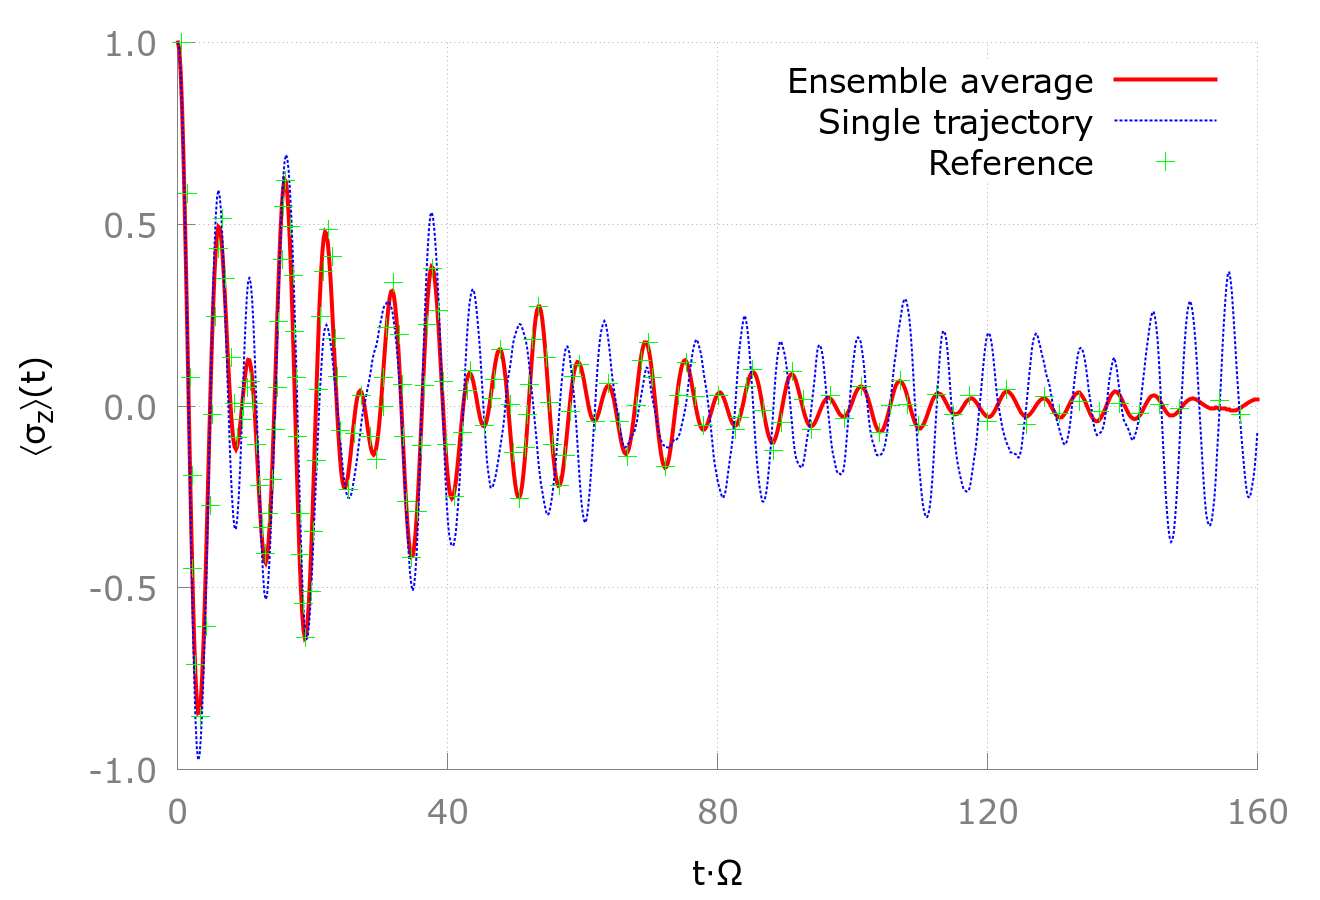
\includegraphics[width=22cm, height=15cm]{nonlin_full.png}
    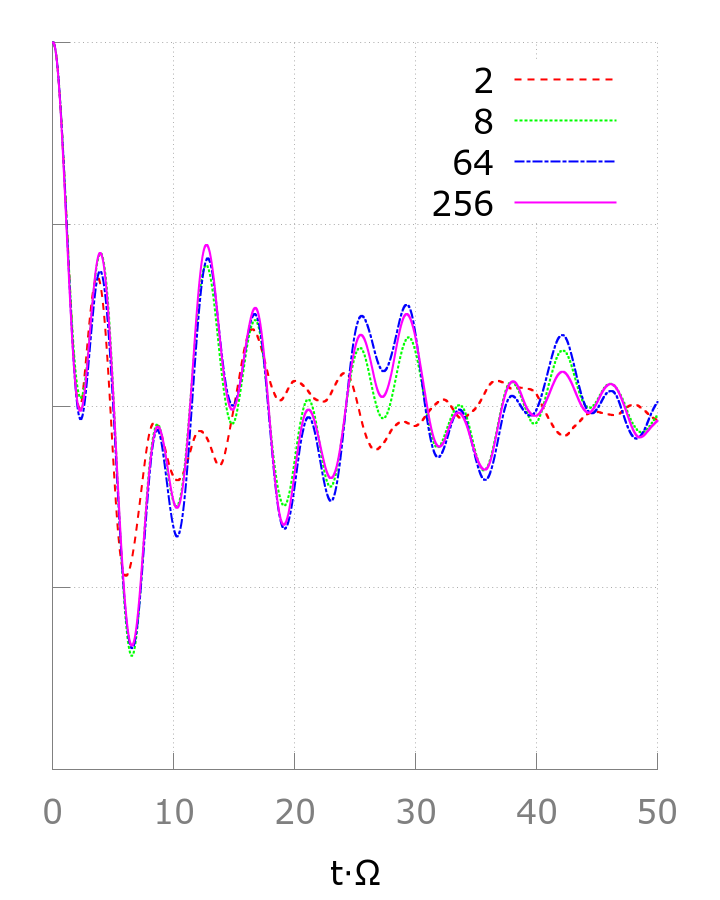
\includegraphics[width=12cm, height=15cm]{nonlin_small.png}
  \end{center} 
  &
  \begin{center}
    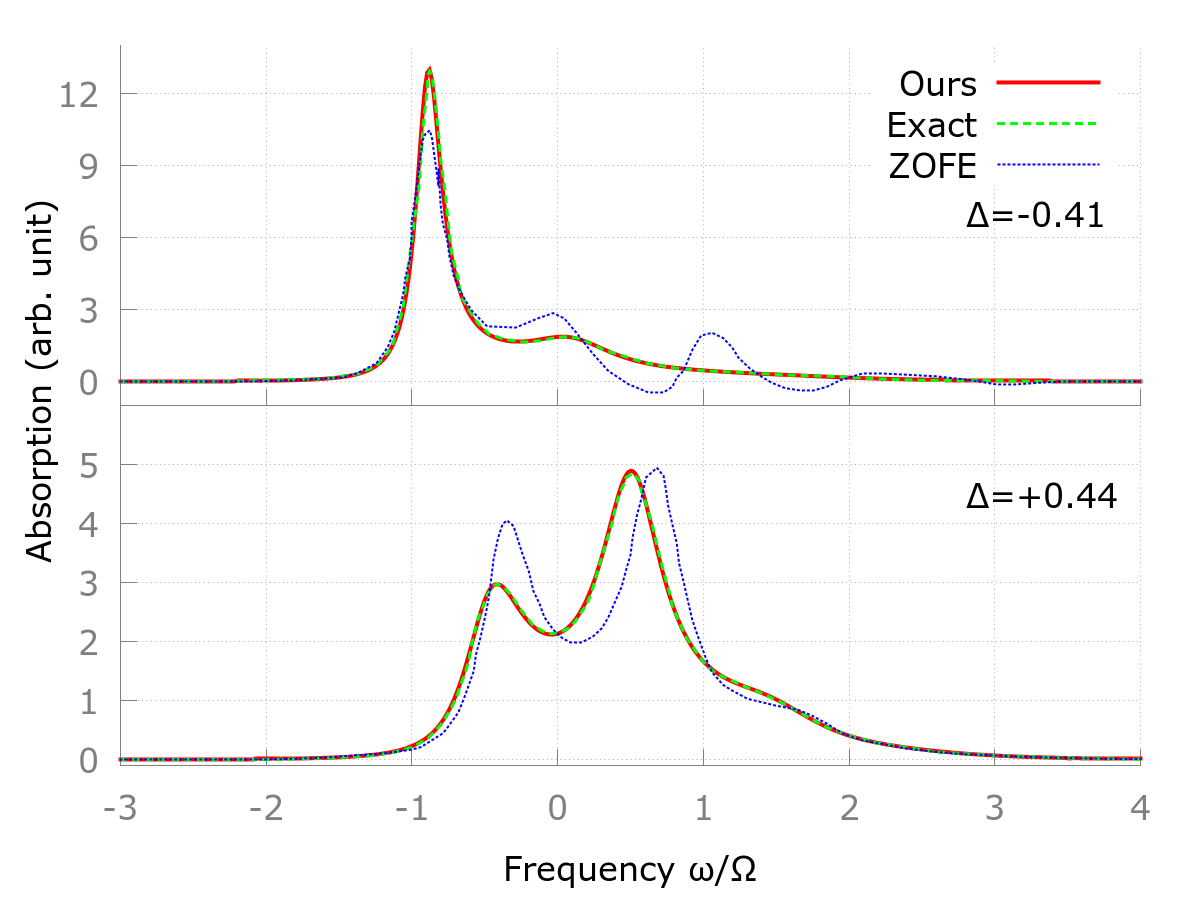
\includegraphics[width=20cm, height=15cm]{spectra.png}
  \end{center}
\end{tabular}
\begin{tabular}{m{0.55\textwidth} m{0.35\textwidth}}
  \begin{description}
    \item[Left picture] Time evolution of weakly coupled Spin-Boson model in highly  non-Markovian regime. Comparison between our approach and the analytical results of [3]. 
    \item[Right picture] Same parameters but stronger coupling. Comparison between different numbers of hierarchies. 
  \end{description}
  &
  Absorption spectra of dimer for two coupling strenghts.
  \textbf{ZOFE} is an ansatz replacing the functional derivative with a time-dependent system operator [4]. Exact calculation is from [4] as well.
\end{tabular}
\end{block}

%}}}
%%%%%%%%%%%%%%%%%%%%%%%%%%%%%%%%%%%%%%%%%%%%%%%%%%%%%%%%%%%%%%%%%%%%%%%%%%%%
%%% Closing Remarks %{{{
%%%%%%%%%%%%%%%%%%%%%%%%%%%%%%%%%%%%%%%%%%%%%%%%%%%%%%%%%%%%%%%%%%%%%%%%%%%%
\setlength{\tabcolsep}{0cm}

\begin{tabular}{p{.55\textwidth} p{.02\textwidth} p{.43\textwidth}}
\begin{block}{Conclusion and outlook}
  \begin{itemize}
    \item efficient tool for small systems $\rightarrow$ apply to larger and more interesting systems
    \item[\raisebox{.2ex}{$\Rightarrow$}] especially the inclusion of thermal noise and more complex spectral densities
    \item further comparison with established approaches (ZOFE [4], Tanimura [1], \dots)
    \item better understanding of the underlying mathematics (e.g.\ of the functional derivative)
  \end{itemize}
\end{block}

&    &

\begin{block_wo_heading}
  \begin{small}
    \begin{description}
    \item \textbf{[1]} \ Y.\ Tanimura, JPSJ \textbf{75}, 8 (2006)
    \item \textbf{[2]} \ L.\ Di�si, N.\ Gisin, W.\ T.\ Strunz, Phys.\ Rev.\ A \textbf{58}, 3 (1998)
    \item \textbf{[3]} \ P.\ Huang, H.\ Zheng, J.\ Phys: Condens.\ Matter \textbf{20}, 395233 (2008)
    \item \textbf{[4]} \ J.\ Roden, W.\ T.\ Strunz, A.\ Eisfeld, J.\ Chem.\ Phys.\ \textbf{134}, 034902 (2011)
  \end{description}
  The author wants to express his gratitude to Gerhard Ritschel and Alexander Eisfeld for providing productive discussion and help with the creation of the spectra-plot. 
  \end{small}
  \vspace{1.55pt}
\end{block_wo_heading}
\end{tabular}

%}}}
\end{document}
